% composite.tex
%
\renewcommand{\thisname}{Chart::Composite}
\section{\thisname}
\name{\thisname}
\file{Composite.pm}
\requires{Chart::Base, GD, Carp, FileHandle}
\begin{Description}
The class \thisclass creates a two component chart with two types of
charts which are layered one above each other. Just set the option
\attruse{composite\_info}. For example, you can create a two component
chart with bars and lines. A composite chart does not make sense with
all combinations of chart types, but it works pretty good with Lines,
Points, LinesPoints and Bars. Note that two similar chart types may come
into visual conflict. \thisclass can do only composite charts made up of
two components. \thisclass is a subclass of \class{Chart::Base}.
\end{Description}

\example
\begin{figure}[ht]
  \begin{center}
    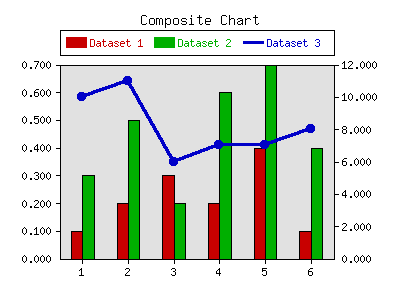
\includegraphics[scale=0.6]{composite.png}
  \end{center}
  \caption{Composite chart}
  \label{fig:composite}
\end{figure}
\begin{verbatim}
use Chart::Composite;

$g = Chart::Composite->new();

$g->add_dataset(1, 2, 3, 4, 5, 6);
$g->add_dataset(0.1, 0.2, 0.3, 0.2, 0.4, 0.1);
$g->add_dataset(0.3, 0.5, 0.2, 0.6, 0.7, 0.4);
$g->add_dataset(10,  11,  6,   7,   7,   8);

$g->set('composite_info' => [ ['Bars',        [1, 2]],
                              ['LinesPoints', [3]  ]
                            ],
        'title'                     => 'Composite Chart',
        'legend'                    => 'top',
        'legend_example_height'     => 'true',
        'legend_example_height0..1' => 10,
        'legend_example_height2'    =>  3,
       );
$g->set('include_zero'  => 'true');

$g->png("composite.png");
\end{verbatim}

\constructorblurb{\thisname}

\attrdecl{brush\_size1}
\begin{AttrDecl}{brush\_size2}
If using component charts having \attruse{brush\_size} as one of their
attributes, you can define the sizes of the brushes individually.
Default is 6 (pixel).
\end{AttrDecl}

\begin{AttrDecl}{composite\_info}
This option is only used for composite charts. It contains the
information which types to use for the two component charts, and which
datasets belong to which component chart. It should be a reference to an
array of array references, containing information like the following:\\
\$obj\deref set ('composite\_info' \fatcomma [ ['Bars', [1,2]], ['Lines', [3,4] ] ]);

This example would set the two component charts to be a bar chart and a
line chart. It would use the first two data sets for the bar chart and
the second two data sets for the line chart. The default is undef. Note
that the numbering starts at 1, not at 0 like most of the other numbered
things in \class{Chart}, because index 0 refers to the $x$ values which
are shared by the two component charts. The ordering of the components
may be important, since the first component is drawn first and then
(partially) overdrawn with the second component. \Eg, when composing a
line graph and a bar graph, it is safer to have the bars in the first
component since otherwise the line(s) might be hidden behind them.
\end{AttrDecl}

\attrdecl{f\_y\_tick1}
\begin{AttrDecl}{f\_y\_tick2}
Needs a reference to a function which uses the $y$ tick labels for the
primary and for the secondary $y$ axis, respectively. These functions
should return a reformatted version of the label as a string. \Eg
\begin{SmallExample}
\$obj\deref set ('f\_y\_tick1' \fatcomma \bs\&formatter1);\\
\$obj\deref set ('f\_y\_tick2' \fatcomma \bs\&formatter2);
\end{SmallExample}
\end{AttrDecl}

\attrdecl{max\_val1}
\begin{AttrDecl}{max\_val2}
Only for composite charts. These options specify the maximum $y$ value
for the first and the second component, respectively. Both default to
undef.
\end{AttrDecl}

\attrdecl{min\_val1}
\begin{AttrDecl}{min\_val2}
Only for composite charts. These options specify the minimum $y$ value
for the first and the second component, respectively. Both default to
undef.
\end{AttrDecl}

\begin{AttrDecl}{legend\_example\_height}
Only for composite charts. This option changes the thickness of the
lines in the legend. If `legend\_example\_height' is set to `true' the
thickness of each legend line can be changed individually. Default is
false. \Eg
\begin{SmallExample}
\$obj\deref set ('legend\_example\_height'     \fatcomma 'true');\\
\$obj\deref set ('legend\_example\_height0'    \fatcomma '3');\\
\$obj\deref set ('legend\_example\_height1..4' \fatcomma '10');
\end{SmallExample}

This example would set the thickness of the first line in the legend to
3, and the thicknesses of the following 4 lines to 10 (using the same
indexing scheme as in `composite\_info'). The default value for each
individual entry is 1, \ie a `normal' line is drawn. It is not possible
to change a 'legend\_example\_height\#'(where \# denotes a dataset
number) which was once defined. (The first setting will remain
unchanged.)
\end{AttrDecl}

\begin{AttrDecl}{same\_y\_axes}
Forces both component charts in a composite chart to use the same
maximum and minimum $y$ values if set to `true'. This helps to keep
some composite charts from being too confusing. Default is undef.
\end{AttrDecl}

\attrdecl{y\_ticks1}
\begin{AttrDecl}{y\_ticks2}
The number of $y$ ticks to use on the primary and on the secondary $y$
axis on a composite chart, respectively. Please note that if you just
set the `y\_ticks' option, both axes will use that number of $y$ ticks.
Both default to undef.
\end{AttrDecl}

\begin{AttrDecl}{flip\_composite\_order}
Flip the drawing order of the components.
Without setting this attribute to true,
the second component will be layered above the first one.
And setting this attribute to true,
the second component will be layered below the first one.
\end{AttrDecl}
